\section{EVD user interface}
\subsection{Log in}
\begin{figure}[H]
    \centering
    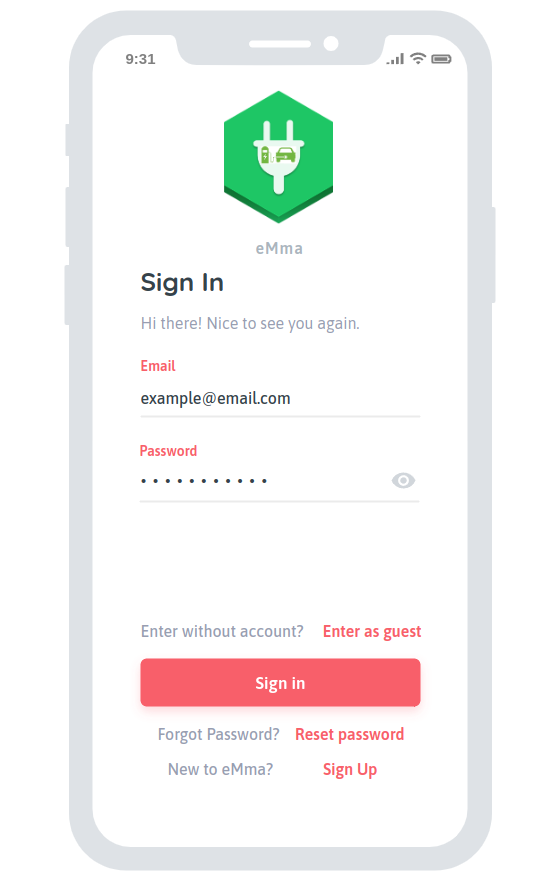
\includegraphics[width=0.4\textwidth]{Images/cp3/logIn.png}
    \caption{UI for the log in}
\end{figure}
We can see from the UI for the log in that the operation is very simple. To sign up is enough to enter the email and the password used during the registration. The EVD can enter into eMma as a guest, if he doesn't want to sign up, but in that case it will perceive only some limited functionalities of the application. It can also be useful to set a mechanism to manage the case in which the user forgets his password.

\subsection{Register}
\begin{figure}[H]
    \centering
    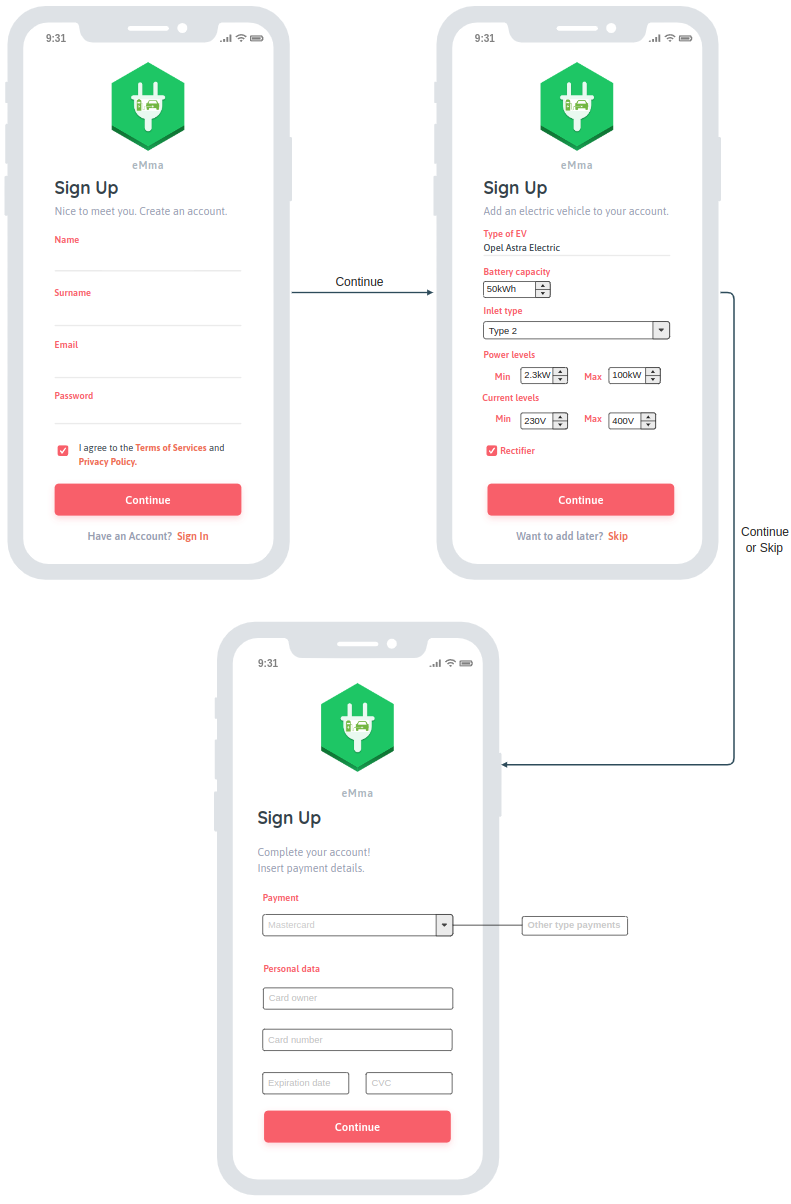
\includegraphics[width=0.85\textwidth]{Images/cp3/registerMockup.png}
    \caption{UI for registration}
\end{figure}
The UI for the registration was thought in order to be as user-friendly as possible. First, to sign up is necessary to insert some personal data, such as the name, the surname, and the email and password that will be used for the log in, as previously explained. It is also necessary to accept the 'Term of Service' in order to continue with the registration. The second step asks the user to add some data about his EV and we can see that the insertion is guided by the interface in order to avoid as much as possible data errors. The EVD has to add the type of the EV, the inlet type, the power levels and the current levels, and has to check or not the final box to inform if the car has or not the rectifier. Finally, to complete the sign up process the user is requested to insert the payment details. After registration, from the personal profile the EVD will be able to add new data to his profile, such as new payment methods and new EVs, and he will be able to modify these ones.

\subsection{Charge now}
\begin{figure}[H]
    \centering
    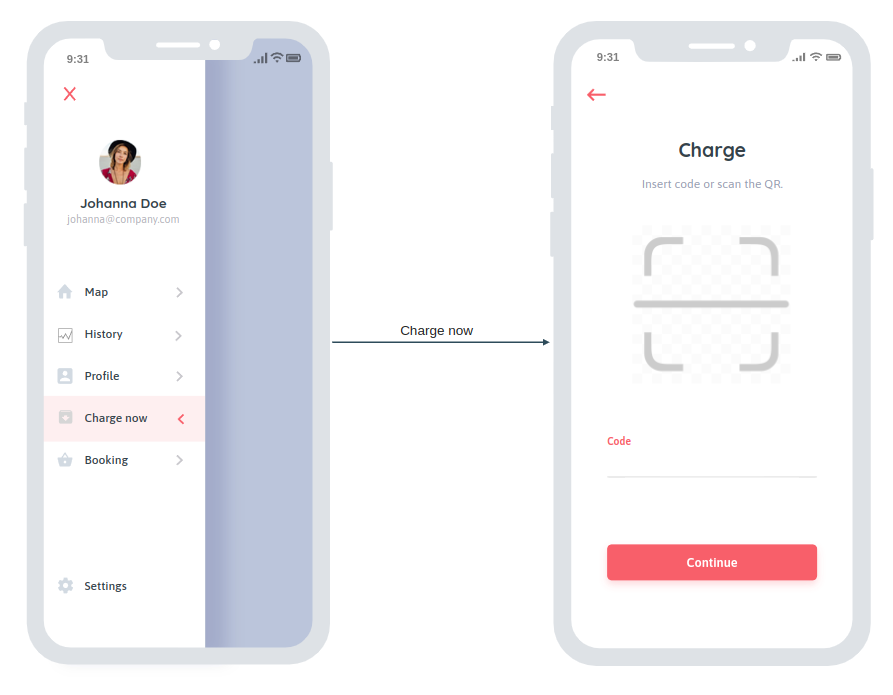
\includegraphics[width=0.85\textwidth]{Images/cp3/chargeNow.png}
    \caption{UI for starting the charging session}
\end{figure}
To start the charging process the EVD has to insert the code or scan the QR present on the charging point. This can be started from the menu or from the 'Charge now' button present in the charging station page, as we will see in the following mock-ups. 

\subsection{Visualize stations}
\begin{figure}[H]
    \centering
    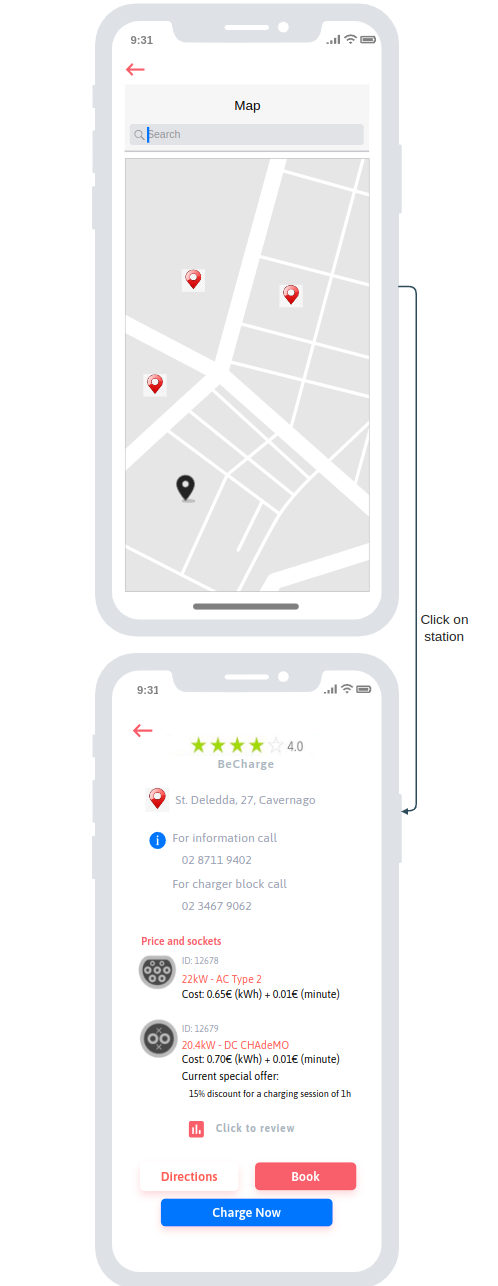
\includegraphics[width=0.4\textwidth]{Images/cp3/visualizeStations.png}
    \caption{UI to visualize stations on the map and their information}
\end{figure}
The main page of the eMma shows to the user the map and permits to visualize the charging stations nearby or to insert a position in which to search for new stations. Clicking on one of the stations, the application shows the charging station page with the most important information: the rating, the name of the station, the address and the contacts, the available sockets and the respective prices and special offers. Finally, it is possible to leave a review or to see the ones left by other users. From this page is possible to get the directions to reach the station and it is also possible to start the main operations of the system: the charging session and the booking of a charging point.

\subsection{Booking charging point}
\begin{figure}[H]
    \centering
    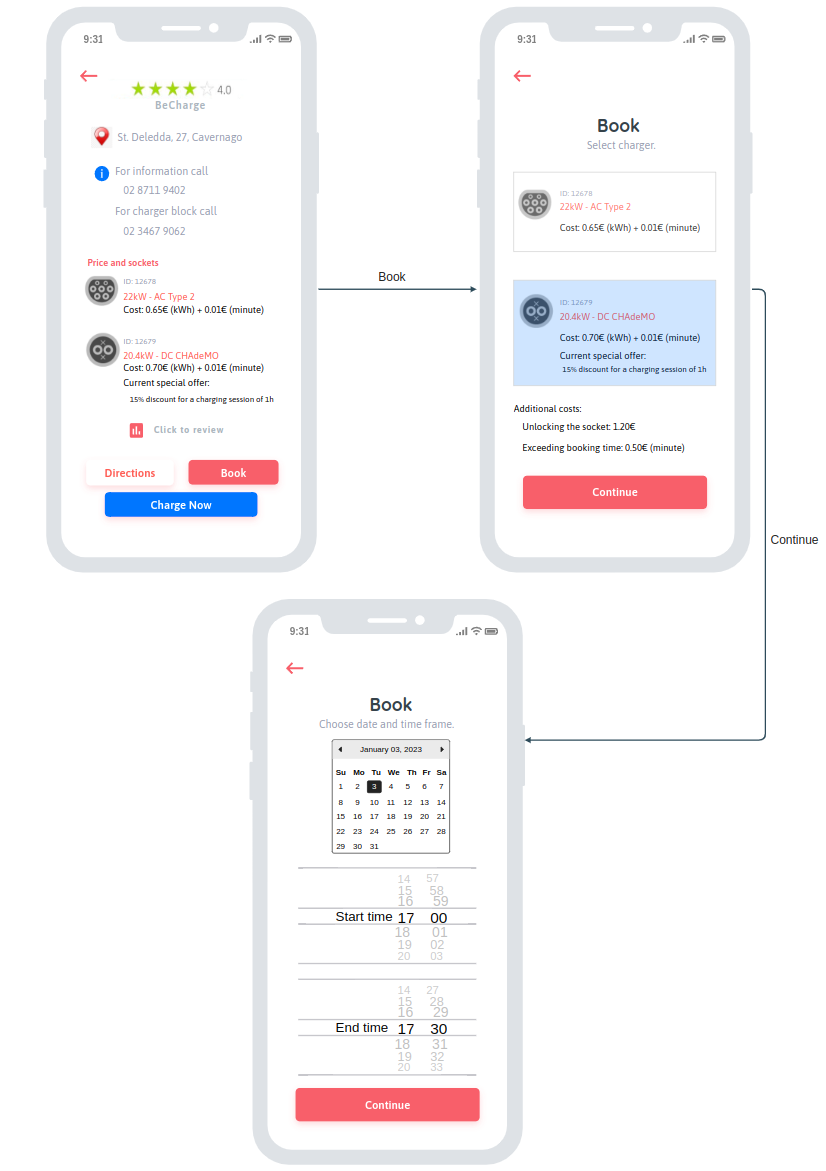
\includegraphics[width=0.75\textwidth]{Images/cp3/bookingCP.png}
    \caption{UI to book the charging point in a certain time frame}
\end{figure}
During the booking operation the EVD has to select the charging point he wants to book from the selected station and also to insert the date and the time frame of the booking. 

\subsection{Terminate charging}
\begin{figure}[H]
    \centering
    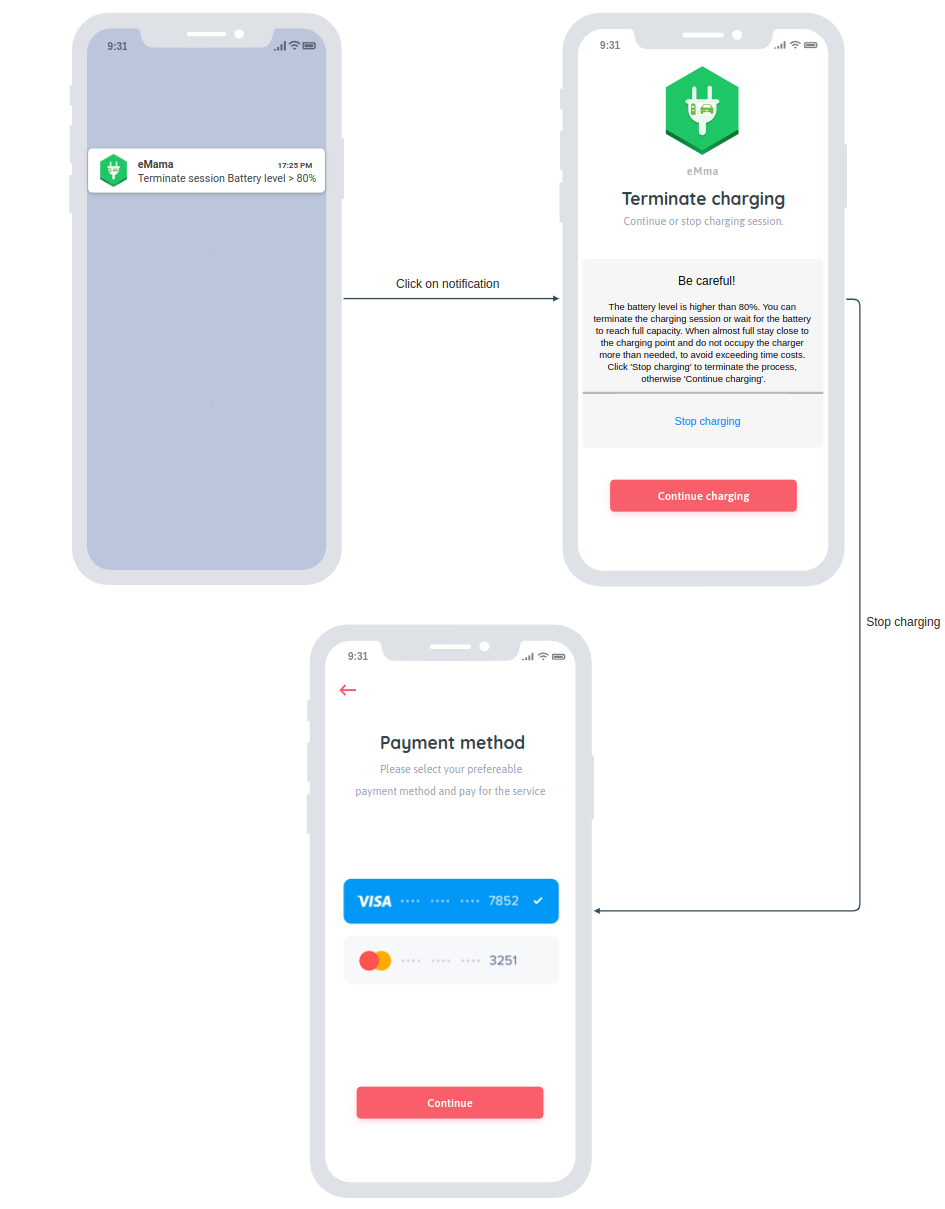
\includegraphics[width=0.9\textwidth]{Images/cp3/terminateCharging.png}
    \caption{UI to terminate the charging session}
\end{figure}
We can see from this UI, that the eMma sends a notification to the user smartphone when the battery level reaches 80\%. The user can decide if he wants to stop the charging session or proceed with the charging until full battery. When the EVD decides to terminate the charging the eMma asks to select the payment method in order to pay for the service.

\clearpage
\section{CPO user interface}